\section{Design}

\subsection{High Level Overview}

The system will comprise 3 parts required to simulate and program a proprietary processor. It will include a virtual machine to emulate the execution of binary machine code catridges, an assembler to translate higher level assembly code into machine code, and finally a compiler for a higher level language to easily program complex applications to run on the processor.

The virtual machine consists of two main processes, the debugger and interpreter. The interpreter will continiously step through memory, decoding and executing instructions sequentially whilst displaying the contents of VRAM through the pixel display.

\shadowbox{
    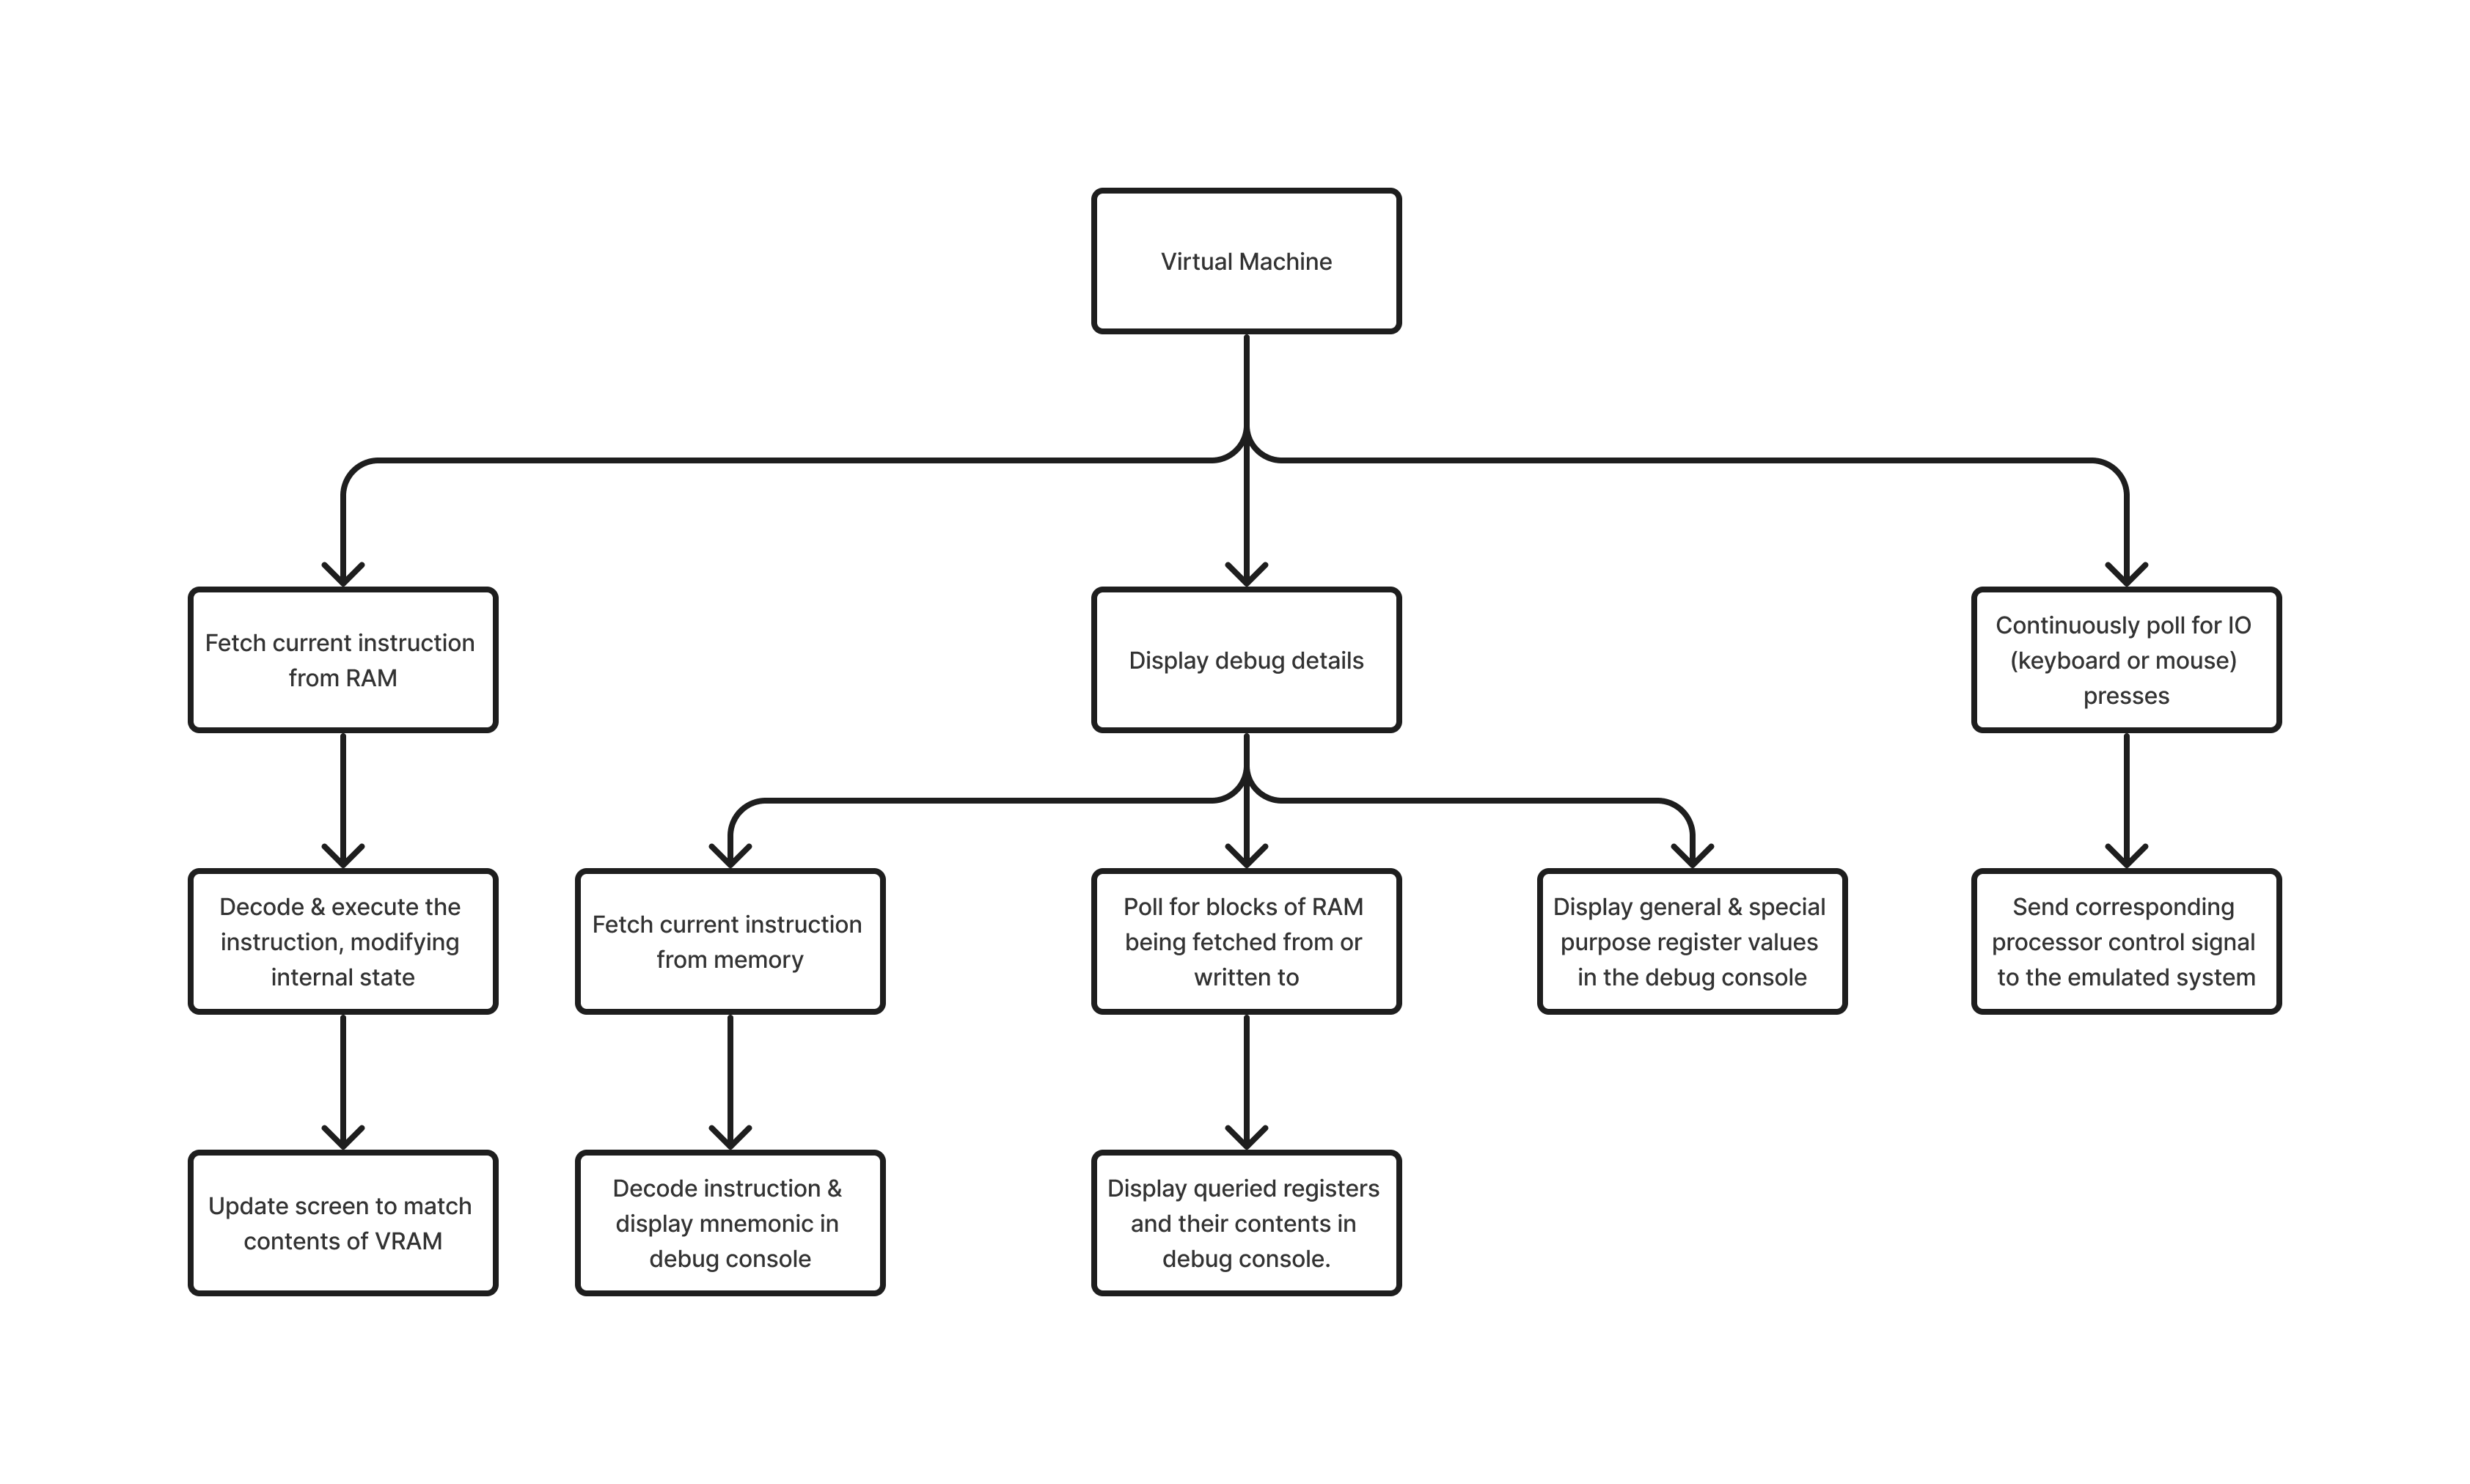
\includegraphics[width=15cm]{Virtual Machine Flowchart.png}
}

\bigskip

The assembler consists of a single pipeline for transforming ASCII assembly programs into binary machine code. The files are loaded into the interpreter which stores their contents in a string. The contents are tokenised and parsed into a sequence of assembly language instructions. These instructions are translated into binary machine code according to the instruction set architecture (defined in \ref{sec:ISADesign}).

\bigskip

\shadowbox{
    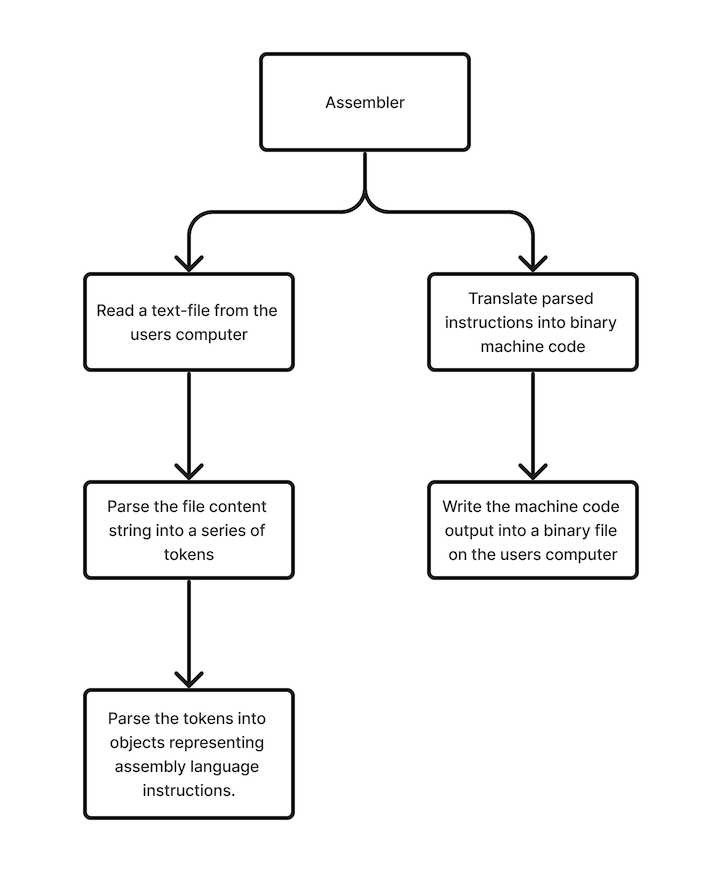
\includegraphics[width=7cm]{Screenshot 2024-06-24 at 19.15.56.png}
}

\bigskip

Much like the assembler, the compiler takes an ASCII program, converts it into tokens and parses it into an Abstract Syntax Tree (AST) representing the structure and order of operations of the program. This AST is converted into an internal representation (IR) designed to help easily locate potential optimisations in the source code (e.g. pre-calculating arithmetic or removing redundant code), these optimisations are made and the IR is converted into an intermediate assembly language due to the presence of high level optimisations such as labels and macro-instructions. Finally, this assembly code is inserted into the assembler and the produced machine code is stored as a file on the users computer. 

\bigskip

\shadowbox{
    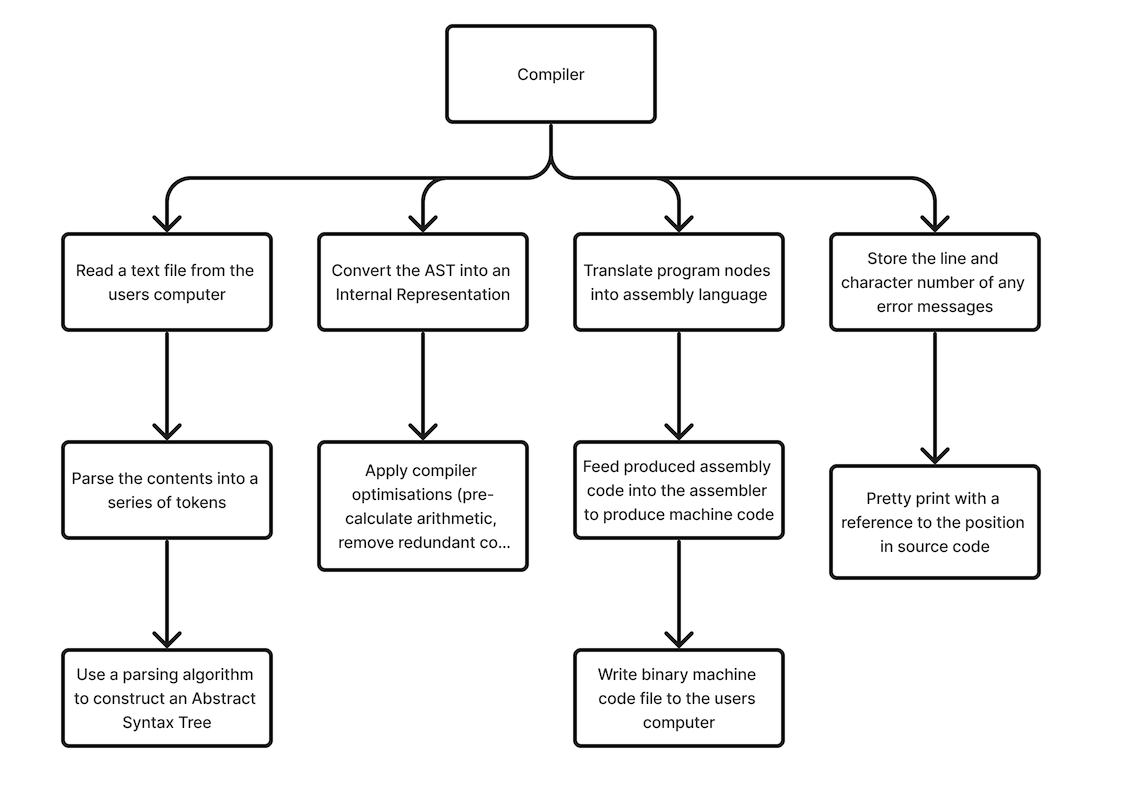
\includegraphics[width=10cm]{Screenshot 2024-06-24 at 19.30.50.png}
}

\subsection{Component Design}
\subsubsection{Instruction Set Architecture}
\label{sec:ISADesign}
The core of any instruction set is the Arithmetic Logic Unit (ALU) so I began by designing an interface for that. There are 2 16-bit inputs to the ALU, which for the purpose of my architecture will only take register values. There are 6 ALU control bits that enable further operations aside from the NOT, AND, and ADD with their own dedicated logic circuits. Different configurations of these control bits can produce various arithmetic operations as detailed in the graphic below.

\bigskip

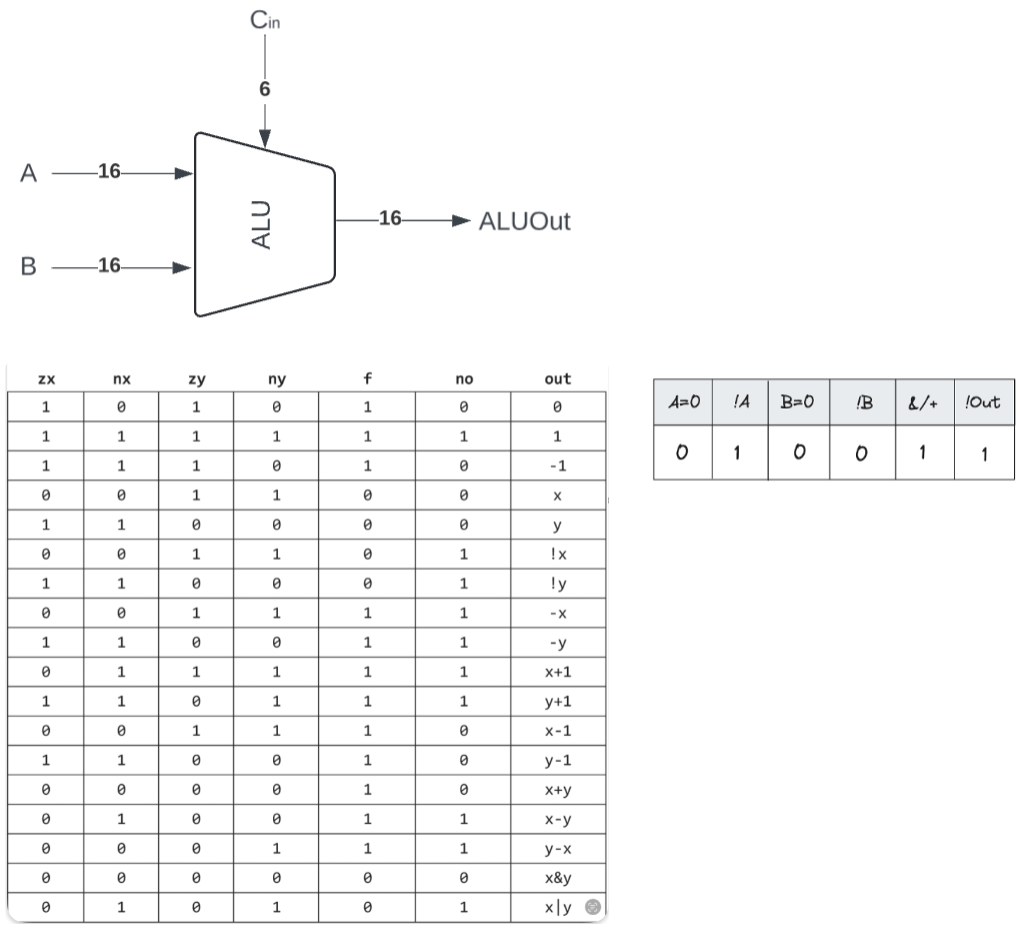
\includegraphics[width=12cm]{Screenshot 2024-07-12 at 16.47.22.png}

\bigskip

I decided to use a MIPS instruction set architecture, minimising the number of instructions supported by the processor. I settled on 3 instruction types: R-type instructions (performing ALU operations on register values), I-type instructions (load and store data between registers and memory), and J-type instructions (conditional jumps to different points in memory). From these 3 types, the following instruction set can be constructed, demonstrated with a program to multiple two numbers stored in memory. (\texttt{'[]'} are used to indicate a memory address):

\begin{lstlisting}[language=C]
R-type: add, sub, and, or, not
I-type: sw, lw
J-type: jmp, jlt, jle, jeq, jge, jgt

// multiply the numbers in memory address 0xb000 and 0xb001, and write the answer to 0xb002
lw r1, [0xb000]
lw r2, [0xb001]

.loop
    // if r2 is 0, break
    li r0, 0
    jle r2, r0, .store

    add r1, r1, r1

    li r0, 1
    sub r2, r2, r0
    jmp .loop

.store
    sw r1, [0xb002]
\end{lstlisting}

\subsubsubsection{ISA Encoding}
Below is the breakdown of how R/I/J type instructions are represented in binary, broken down into their respective fields. All instructions have a 2-bit opcode which dictates the type of instruction, however only 3 instructions types are defined - leaving the fourth configuration to represent a \texttt{NOP} or \texttt{HALT} instruction. The next 6 bits of the R-type instruction are occupied by the ALU control bits which dictate the operation to be carried out. This is followed by two source registers (inputs to the ALU) and the destination register.

After the I-type opcode, an additional bit dictates whether the instruction is to be a load word (lw) or store word (sw). With a subsequent bit determining whether (for a load word instruction) the source value will be an immediate number, or the corresponding memory address (immediate or RAM[immediate]). Similarly for a store word instruction the next bit dictates whether the immediate field specifies a register holding the address in RAM, or an address by itself (RAM[register], RAM[immediate]).  

Finally, for a J-type instruction 3 bits are used to specify the jump condition (>, =, <) combinations of these bits can produce any condition (e.g. 101: !=, 011: <=). Following these there are two source registers used as inputs to the ALU for the comparison, and a 16 bit memory address to jump to should the condition be met. 

\bigskip

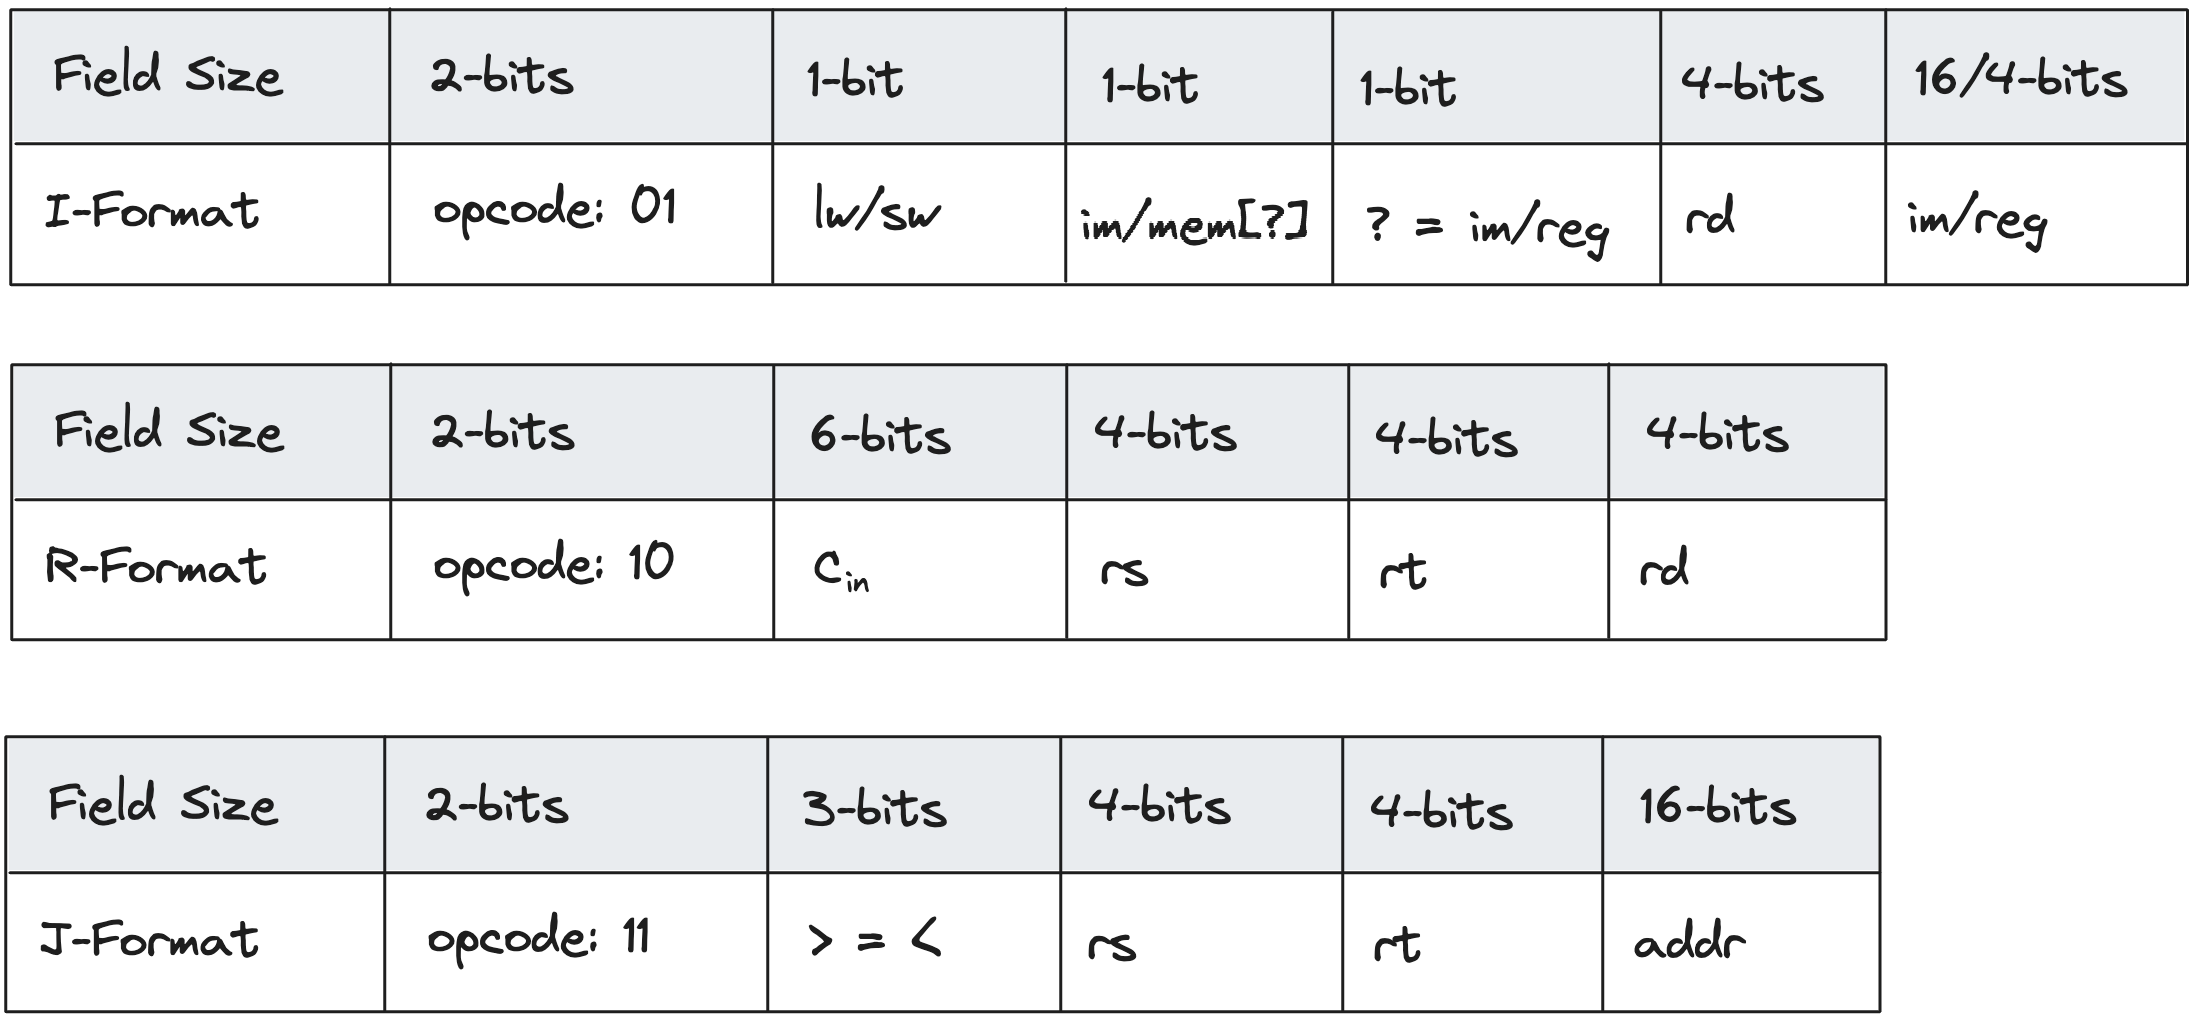
\includegraphics[width=12cm]{Screenshot 2024-07-12 at 23.35.53.png}

\begin{lstlisting}
li r5, 14
lw r4, [0xb000]
sub r6, r5, r4
jge r6, r4, [0x0101]

01 000 0101 00000000 00001110
01 010 0100 10110000 00000000
10 010011 0101 0100 0110
11 110 0110 0100 00000001 00000001
\end{lstlisting}

\subsection{Virtual Machine}
\subsubsection{Data Structures}
\subsubsection{Algorithms}